\begin{document}
\lstset{language=suiterc}

\section{Cylc Introduction}


\subsection{The suite.rc File}

A cylc suite is a collection of files located within a directory called the
suite directory, the suite is configured by a single suite.rc file.
The suite.rc file uses a nested INI based format where sections are denoted
by square brackets, sub-sections by double square brackets and
sub-sub-sections by triple square brackets.

\begin{lstlisting}[language=suiterc]
[section]
    [[subsection]]
        option = value
\end{lstlisting}

There are five top level sections that can be present in a suite.rc file, the
three main ones are:

\begin{description}
\item[{[cylc]}] Used for suite-level configuration.
\item[{[scheduling]}] Defines the logic of the suite enabling cylc to determine
when tasks are ready to run.
\item[{[runtime]}] Defines the tasks themselves, what to execute, where and how.
\end{description}


\subsection{Hello World in cylc}

The simplest working example of a cylc suite is given below, this suite
contains a single task named hello\_world which waits 5 seconds then outputs
the text ``Hello World!'' to standard out. The task is defined in in the
\lstinline=[runtime]= section and cylc is told to run the task by the
\lstinline[mathescape]=graph $=$ hello_world= part.

\begin{lstlisting}[language=suiterc]
[scheduling]
    [[dependencies]]
        graph = hello_world
[runtime]
    [[hello_world]]
        script = sleep 5; echo "Hello World!"
\end{lstlisting}

To run new a suite there are three things that must be done, firstly the suite
must be registered with cylc, then (optionally) we can validate the suite to
ensure there are no errors in the suite.rc file. Finally we can run the suite.
These steps can be undertaken on the command line like:

\begin{lstlisting}[mathescape, language=bash]
$\$$ cylc register hello_world /path/to/suite/
$\$$ cylc validate hello_world
$\$$ cylc run hello_world
\end{lstlisting}

For simplicity \lstinline=rose suite-run= command does all of this for us,
though in order to operate it requires a rose-suite.conf file which should sit
alongside the suite.rc file. The rose-suite.conf file can be empty.

\begin{lstlisting}[mathescape, language=bash]
$\$$ rose suite-run
\end{lstlisting}

\paragraph*{Demo}
To run the hello world example, create a directory called hello\_world, this
will be our suite directory.

Next copy the example code into a suite.rc file within that directory.

Finally run the following commands:

\begin{lstlisting}[mathescape, language=bash]
$\$$ cd hello_world  # move to the suite directory
$\$$ touch rose-suite.conf  # create an empty rose-suite.conf file
$\$$ rose suite-run  # run the suite
\end{lstlisting}

If successful cylc will generate some output then a window will open. This is
the cylc gui, the tool that displays the current status of your suite. In the
cylc gui you should briefly see the task hello\_world displayed with a coloured
square next to it. The colour of the square represents the state of the task
(for example green means the task is running and gray that it has succeeded).
Once the hello\_world task has succeeded, having no more tasks to run the suite
will automatically shut down.


\subsection{Tasks}

To convert a script into a cylc task the script should be placed inside a
`bin` directory alongside the suite.rc file in the suite directory.

\begin{lstlisting}[language=]
suite-directory/
|-- bin/
|   `-- get-host-details
`-- suite.rc
\end{lstlisting}

The script can then be referenced in the suite.rc file e.g.:

\begin{lstlisting}[language=suiterc]
[scheduling]
    [[get_info]]
        script = get-host-details
\end{lstlisting}

In the task definition it is possible to determine what the task will run, as
well as where and how the task will run. For example by adding a
\lstinline=[[[remote]]]= section to the task definition it is possible to
specify the host that will run the command e.g.:

\begin{lstlisting}[language=suiterc]
[scheduling]
    [[get_info]]
        script = get-host-details
        [[[remote]]]
            host = supercomputer
\end{lstlisting}

It is also possible to pass information to the script, for instance in the
following example the script ``get-host-details'' is provided with the
environment variable ``FOO'' set to ``bar''.

\begin{lstlisting}[language=suiterc]
[scheduling]
    [[get_info]]
        script = get-host-details
        [[[environment]]]
            FOO = bar
\end{lstlisting}


\subsection{Graphs}

The hello\_world suite contained the line
\lstinline[mathescape]=graph $=$ hello_world=, this is a graph string. In cylc
graph strings contain the logic for determining when tasks can be run. A graph
string should contain a list of tasks along with the inter-dependence between
them. For instance if we have two tasks foo and bar, where foo is
dependent on bar succeeding, then we would this logic in a graph string as:

\begin{lstlisting}[language=suiterc]
graph = foo => bar
\end{lstlisting}

This graph string tells cylc to run foo and then once foo has succeeded run
bar. Note that if foo fails bar will not run. These relationships are called
dependencies, a graph string can contain multiple dependencies.

\begin{lstlisting}[language=suiterc]
graph = """
    foo => bar
    bar => baz
    bar => qux
    baz => pin
    qux => pin
    wol
"""
\end{lstlisting}

\note{The graph string can be written over multiple lines using
triple, double quotation marks (\lstinline="""=).}

The logic of the previous graph string is outlined in the following diagram.

\begin{center}
    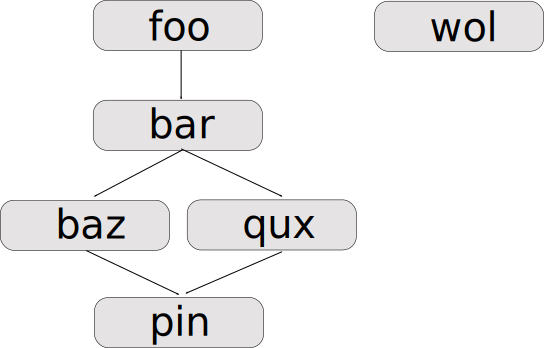
\includegraphics[width=0.4\columnwidth]{resources/tex/cylc-graph}
\end{center}


\subsection{Cycling}

Graph strings allow us to define workflows consisting of tasks. In a suite we
may well want to repeat workflows, which is called cycling.

\begin{center}
    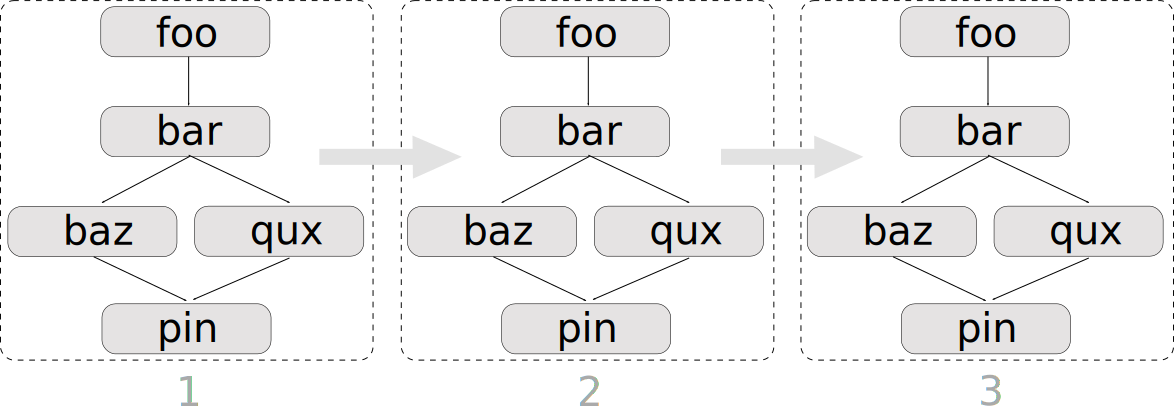
\includegraphics[width=0.6\columnwidth]{resources/tex/cylc-cycle-graph}
\end{center}

The above diagram shows the workflow from the previous example repeated three
times with the resultant cycles numbered 1, 2 and 3. With cylc cycles can
either be numbered or alternatively can use datetimes, for this tutorial shall
use datetimes.

In order to cycle a workflow we need a start point to begin cycling from, and
end point to finish cycling at. In cylc these are defined using the
\lstinline=initial cycle point= and \lstinline=final cycle point= values which
are set in the \lstinline=[scheduling]= section.

We tell cylc to cycle over a workflow using graph headers. A graph header is a
section that sits inside the \lstinline=[[dependencies]]= section. In the
following example the task foo will run once every day at midday starting on
the 1st of January 2000 and ending on the 5th of January 2000.

\begin{lstlisting}[language=suiterc]
[scheduling]
    initial cycle point = 2000-01-01T00
    final cycle point = 2000-01-05T00
    [[dependencies]]
        [[[T12]]]
            graph = foo
\end{lstlisting}

In this example the graph header \lstinline=[[[T12]]]= means run the workflow
defined in the \lstinline=graph= section once every day at 12:00. Equally
\lstinline=[[[T06]]]= means run every day at 06:00 and \lstinline=[[[T2145]]]=
means run every day at 21:45.

\note{When we talk of tasks running every day we don't mean that
the suite waits an entire day before running the next task, cycle points are
just labels we can use to organise cycles. It is possible to set real-world
datetimes as dependencies for cylc tasks see the \textbf{TODO: link to advanced
section: wallclock}.}

There are multiple forms of graph header to serve different purposes, more
exotic forms are outlined in \textbf{TODO: link to advanced section graph
headers}.

\paragraph*{Demo}
This demo is an example of a cycling workflow, to run it create a new
directory and create a blank rose-suite.conf file within it.

Next copy the following code into a suite.rc and a bin/count-down file.

\begin{lstlisting}[language=]
|-- bin/
|   `-- count-down
|-- rose-suite.conf
`-- suite.rc
\end{lstlisting}

\begin{lstlisting}[language=suiterc, title=suite.rc]
[scheduling]
    max active cycle points = 1  # To keep the next cycle from running before
                                 # the current one has finished.
    initial cycle point = 2000-01-01T00
    final cycle point = 2000-01-05T00
    [[dependencies]]
        [[[T00]]]
            graph = """
                point_upwards => load_astronauts
                point_upwards => fill_fuel_tank
                point_upwards => set_coordinates
                fill_fuel_tank => light_fuse
                set_coordinates => count_down
                light_fuse => count_down
                load_astronauts => count_down
                count_down => blast_off
            """
[runtime]
    [[point_upwards]]
        script = sleep 2; echo "spikey end pointing at sky, flamey end \
                    pointing at ground"
    [[load_astronauts]]
        script = sleep 1; echo "loaded astronauts"
    [[fill_fuel_tank]]
        script = sleep 5; echo "tank brimmed"
    [[set_coordinates]]
        script = echo "coordinates set for west wallaby st"
    [[light_fuse]]
        script = echo "stand well back"
    [[count_down]]
        script = count-down
    [[blast_off]]
        script = echo "blast off"
\end{lstlisting}

\begin{lstlisting}[language=bash, title=bin/count-down]
sleep 1; echo 5;
sleep 1; echo 4;
sleep 1; echo 3;
sleep 1; echo 2;
sleep 1; echo 1;
\end{lstlisting}

To run this demo suite, enter the following commands:

\begin{lstlisting}[language=bash, mathescape]
$\$$ chmod +x bin/count-down  # Make the count-down script executable.
$\$$ rose suite-run
\end{lstlisting}

Again a window should open up showing you the progress of the suite.
Whilst the suite is running try entering graph mode by selecting
\lstinline[language=]{View > 1 - Graph View} from the menubar, this will show
the dependencies between the tasks as they run.


\subsection{Inter Cycle Dependence}

TODO: Brief explanation of inter-cycle dependencies.


\end{document}
